%%%%%%%%%%%%%%%%%%%%%%%%%%%%%%%%%%%%%%%%%%%%%%%%%%%%%%%%%%%%%%%%%%%%%%
% Template for a UBC-compliant dissertation
% At the minimum, you will need to change the information found
% after the "Document meta-data"
%
%!TEX TS-program = pdflatex
%!TEX encoding = UTF-8 Unicode

%% The ubcdiss class provides several options:
%%   gpscopy (aka fogscopy)
%%       set parameters to exactly how GPS specifies
%%         * single-sided
%%         * page-numbering starts from title page
%%         * the lists of figures and tables have each entry prefixed
%%           with 'Figure' or 'Table'
%%       This can be tested by `\ifgpscopy ... \else ... \fi'
%%   10pt, 11pt, 12pt
%%       set default font size
%%   oneside, twoside
%%       whether to format for single-sided or double-sided printing
%%   balanced
%%       when double-sided, ensure page content is centred
%%       rather than slightly offset (the default)
%%   singlespacing, onehalfspacing, doublespacing
%%       set default inter-line text spacing; the ubcdiss class
%%       provides \textspacing to revert to this configured spacing
%%   draft
%%       disable more intensive processing, such as including
%%       graphics, etc.
%%

% For submission to GPS
\documentclass[gpscopy,onehalfspacing,11pt]{ubcdiss}

% For your own copies (looks nicer)
% \documentclass[balanced,twoside,11pt]{ubcdiss}

%%%%%%%%%%%%%%%%%%%%%%%%%%%%%%%%%%%%%%%%%%%%%%%%%%%%%%%%%%%%%%%%%%%%%%
%%%%%%%%%%%%%%%%%%%%%%%%%%%%%%%%%%%%%%%%%%%%%%%%%%%%%%%%%%%%%%%%%%%%%%
%%
%% FONTS:
%% 
%% The defaults below configures Times Roman for the serif font,
%% Helvetica for the sans serif font, and Courier for the
%% typewriter-style font.  Configuring fonts can be time
%% consuming; we recommend skipping to END FONTS!
%% 
%% If you're feeling brave, have lots of time, and wish to use one
%% your platform's native fonts, see the commented out bits below for
%% XeTeX/XeLaTeX.  This is not for the faint at heart. 
%% (And shouldn't you be writing? :-)
%%

%% NFSS font specification (New Font Selection Scheme)
\usepackage{times,mathptmx,courier}
\usepackage[scaled=.92]{helvet}

%% Math or theory people may want to include the handy AMS macros
%\usepackage{amssymb}
%\usepackage{amsmath}
%\usepackage{amsfonts}

%% The pifont package provides access to the elements in the dingbat font.   
%% Use \ding{##} for a particular dingbat (see p7 of psnfss2e.pdf)
%%   Useful:
%%     51,52 different forms of a checkmark
%%     54,55,56 different forms of a cross (saltyre)
%%     172-181 are 1-10 in open circle (serif)
%%     182-191 are 1-10 black circle (serif)
%%     192-201 are 1-10 in open circle (sans serif)
%%     202-211 are 1-10 in black circle (sans serif)
%% \begin{dinglist}{##}\item... or dingautolist (which auto-increments)
%% to create a bullet list with the provided character.
\usepackage{pifont}

%%%%%%%%%%%%%%%%%%%%%%%%%%%%%%%%%%%%%%%%%%%%%%%%%%%%%%%%%%%%%%%%%%%%%%
%% Configure fonts for XeTeX / XeLaTeX using the fontspec package.
%% Be sure to check out the fontspec documentation.
%\usepackage{fontspec,xltxtra,xunicode}	% required
%\defaultfontfeatures{Mapping=tex-text}	% recommended
%% Minion Pro and Myriad Pro are shipped with some versions of
%% Adobe Reader.  Adobe representatives have commented that these
%% fonts can be used outside of Adobe Reader.
%\setromanfont[Numbers=OldStyle]{Minion Pro}
%\setsansfont[Numbers=OldStyle,Scale=MatchLowercase]{Myriad Pro}
%\setmonofont[Scale=MatchLowercase]{Andale Mono}

%% Other alternatives:
%\setromanfont[Mapping=tex-text]{Adobe Caslon}
%\setsansfont[Scale=MatchLowercase]{Gill Sans}
%\setsansfont[Scale=MatchLowercase,Mapping=tex-text]{Futura}
%\setmonofont[Scale=MatchLowercase]{Andale Mono}
%\newfontfamily{\SYM}[Scale=0.9]{Zapf Dingbats}
%% END FONTS
%%%%%%%%%%%%%%%%%%%%%%%%%%%%%%%%%%%%%%%%%%%%%%%%%%%%%%%%%%%%%%%%%%%%%%
%%%%%%%%%%%%%%%%%%%%%%%%%%%%%%%%%%%%%%%%%%%%%%%%%%%%%%%%%%%%%%%%%%%%%%



%%%%%%%%%%%%%%%%%%%%%%%%%%%%%%%%%%%%%%%%%%%%%%%%%%%%%%%%%%%%%%%%%%%%%%
%%%%%%%%%%%%%%%%%%%%%%%%%%%%%%%%%%%%%%%%%%%%%%%%%%%%%%%%%%%%%%%%%%%%%%
%%
%% Recommended packages
%%
\usepackage{checkend}	% better error messages on left-open environments
\usepackage{graphicx}	% for incorporating external images

%% booktabs: provides some special commands for typesetting tables as used
%% in excellent journals.  Ignore the examples in the Lamport book!
\usepackage{booktabs}

%% listings: useful support for including source code listings, with
%% optional special keyword formatting.  The \lstset{} causes
%% the text to be typeset in a smaller sans serif font, with
%% proportional spacing.
\usepackage{listings}
\lstset{basicstyle=\sffamily\scriptsize,showstringspaces=false,fontadjust}

%% The acronym package provides support for defining acronyms, providing
%% their expansion when first used, and building glossaries.  See the
%% example in glossary.tex and the example usage throughout the example
%% document.
%% NOTE: to use \MakeTextLowercase in the \acsfont command below,
%%   we *must* use the `nohyperlinks' option -- it causes errors with
%%   hyperref otherwise.  See Section 5.2 in the ``LaTeX 2e for Class
%%   and Package Writers Guide'' (clsguide.pdf) for details.
\usepackage[printonlyused,nohyperlinks]{acronym}
%% The ubcdiss.cls loads the `textcase' package which provides commands
%% for upper-casing and lower-casing text.  The following causes
%% the acronym package to typeset acronyms in small-caps
%% as recommended by Bringhurst.
\renewcommand{\acsfont}[1]{{\scshape \MakeTextLowercase{#1}}}

%% color: add support for expressing colour models.  Grey can be used
%% to great effect to emphasize other parts of a graphic or text.
%% For an excellent set of examples, see Tufte's "Visual Display of
%% Quantitative Information" or "Envisioning Information".
\usepackage{color}
\definecolor{greytext}{gray}{0.5}

%% comment: provides a new {comment} environment: all text inside the
%% environment is ignored.
%%   \begin{comment} ignored text ... \end{comment}
\usepackage{comment}

%% The natbib package provides more sophisticated citing commands
%% such as \citeauthor{} to provide the author names of a work,
%% \citet{} to produce an author-and-reference citation,
%% \citep{} to produce a parenthetical citation.
%% We use \citeeg{} to provide examples
\usepackage[numbers,sort&compress]{natbib}
\newcommand{\citeeg}[1]{\citep[e.g.,][]{#1}}

%% The titlesec package provides commands to vary how chapter and
%% section titles are typeset.  The following uses more compact
%% spacings above and below the title.  The titleformat that follow
%% ensure chapter/section titles are set in singlespace.
\usepackage[compact]{titlesec}
\titleformat*{\section}{\singlespacing\raggedright\bfseries\Large}
\titleformat*{\subsection}{\singlespacing\raggedright\bfseries\large}
\titleformat*{\subsubsection}{\singlespacing\raggedright\bfseries}
\titleformat*{\paragraph}{\singlespacing\raggedright\itshape}

%% The caption package provides support for varying how table and
%% figure captions are typeset.
\usepackage[format=hang,indention=-1cm,labelfont={bf},margin=1em]{caption}

%% url: for typesetting URLs and smart(er) hyphenation.
%% \url{http://...} 
\usepackage{url}
\urlstyle{sf}	% typeset urls in sans-serif


%%%%%%%%%%%%%%%%%%%%%%%%%%%%%%%%%%%%%%%%%%%%%%%%%%%%%%%%%%%%%%%%%%%%%%
%%%%%%%%%%%%%%%%%%%%%%%%%%%%%%%%%%%%%%%%%%%%%%%%%%%%%%%%%%%%%%%%%%%%%%
%%
%% Possibly useful packages: you may need to explicitly install
%% these from CTAN if they aren't part of your distribution;
%% teTeX seems to ship with a smaller base than MikTeX and MacTeX.
%%
%\usepackage{pdfpages}	% insert pages from other PDF files
%\usepackage{longtable}	% provide tables spanning multiple pages
%\usepackage{chngpage}	% support changing the page widths on demand
%\usepackage{tabularx}	% an enhanced tabular environment

%% enumitem: support pausing and resuming enumerate environments.
%\usepackage{enumitem}

%% rotating: provides two environments, sidewaystable and sidewaysfigure,
%% for typesetting tables and figures in landscape mode.  
%\usepackage{rotating}

%% subfig: provides for including subfigures within a figure,
%% and includes being able to separately reference the subfigures.
%\usepackage{subfig}

%% ragged2e: provides several new new commands \Centering, \RaggedLeft,
%% \RaggedRight and \justifying and new environments Center, FlushLeft,
%% FlushRight and justify, which set ragged text and are easily
%% configurable to allow hyphenation.
%\usepackage{ragged2e}

%% The ulem package provides a \sout{} for striking out text and
%% \xout for crossing out text.  The normalem and normalbf are
%% necessary as the package messes with the emphasis and bold fonts
%% otherwise.
%\usepackage[normalem,normalbf]{ulem}    % for \sout

%%%%%%%%%%%%%%%%%%%%%%%%%%%%%%%%%%%%%%%%%%%%%%%%%%%%%%%%%%%%%%%%%%%%%%
%% HYPERREF:
%% The hyperref package provides for embedding hyperlinks into your
%% document.  By default the table of contents, references, citations,
%% and footnotes are hyperlinked.
%%
%% Hyperref provides a very handy command for doing cross-references:
%% \autoref{}.  This is similar to \ref{} and \pageref{} except that
%% it automagically puts in the *type* of reference.  For example,
%% referencing a figure's label will put the text `Figure 3.4'.
%% And the text will be hyperlinked to the appropriate place in the
%% document.
%%
%% Generally hyperref should appear after most other packages

%% The `pagebackref' causes the references in the bibliography to have
%% back-references to the citing page; `backref' puts the citing section
%% number.  See further below for other examples of using hyperref.
%% 2009/12/09: now use `linktocpage' (Jacek Kisynski): GPS now prefers
%%   that the ToC, LoF, LoT place the hyperlink on the page number,
%%   rather than the entry text.
\ifgpscopy
  % GPS requires that weblinks should be dark blue, which looks a bit
  % odd in printed form.
  % https://www.grad.ubc.ca/current-students/dissertation-thesis-preparation/fonts-print
  \usepackage[bookmarks,bookmarksnumbered,%
     pagebackref,linktocpage,%
     colorlinks=true,%
     linkcolor=black,%
     urlcolor=blue,%
     citecolor=black%
     ]{hyperref}
\else
  %% The following puts hyperlinks in very faint grey boxes (in pdf only).
  \usepackage[bookmarks,bookmarksnumbered,%
    pagebackref,linktocpage,%
    allbordercolors={0.8 0.8 0.8},%
    ]{hyperref}
\fi
%% The following change how the the back-references text is typeset in a
%% bibliography when `backref' or `pagebackref' are used
%%
%% Change \nocitations if you'd like some text shown where there
%% are no citations found (e.g., pulled in with \nocite{xxx})
\newcommand{\nocitations}{\relax}
%%\newcommand{\nocitations}{No citations}
%%
%\renewcommand*{\backref}[1]{}% necessary for backref < 1.33
\renewcommand*{\backrefsep}{,~}%
\renewcommand*{\backreftwosep}{,~}% ', and~'
\renewcommand*{\backreflastsep}{,~}% ' and~'
\renewcommand*{\backrefalt}[4]{%
\textcolor{greytext}{\ifcase #1%
\nocitations%
\or
\(\rightarrow\) page #2%
\else
\(\rightarrow\) pages #2%
\fi}}


%% The following uses most defaults, which causes hyperlinks to be
%% surrounded by colourful boxes; the colours are only visible in
%% PDFs and don't show up when printed:
%\usepackage[bookmarks,bookmarksnumbered]{hyperref}

%% The following disables the colourful boxes around hyperlinks.
%\usepackage[bookmarks,bookmarksnumbered,pdfborder={0 0 0}]{hyperref}

%% The following disables all hyperlinking, but still enabled use of
%% \autoref{}
%\usepackage[draft]{hyperref}

%% The following commands causes chapter and section references to
%% uppercase the part name.
\renewcommand{\chapterautorefname}{Chapter}
\renewcommand{\sectionautorefname}{Section}
\renewcommand{\subsectionautorefname}{Section}
\renewcommand{\subsubsectionautorefname}{Section}

%% New Theorems
\newtheorem{assumption}{Assumption}
\newtheorem{proposition}{Proposition}
\newtheorem{definition}{Definition}
\newtheorem{corollary}{Corollary}
\newtheorem{theorem}{Theorem}
\newtheorem{lemma}{Lemma}

%% If you have long page numbers (e.g., roman numbers in the 
%% preliminary pages for page 28 = xxviii), you might need to
%% uncomment the following and tweak the \@pnumwidth length
%% (default: 1.55em).  See the tocloft documentation at
%% http://www.ctan.org/tex-archive/macros/latex/contrib/tocloft/
% \makeatletter
% \renewcommand{\@pnumwidth}{3em}
% \makeatother

%%%%%%%%%%%%%%%%%%%%%%%%%%%%%%%%%%%%%%%%%%%%%%%%%%%%%%%%%%%%%%%%%%%%%%
%%%%%%%%%%%%%%%%%%%%%%%%%%%%%%%%%%%%%%%%%%%%%%%%%%%%%%%%%%%%%%%%%%%%%%
%%
%% Some special settings that controls how text is typeset
%%
% \raggedbottom		% pages don't have to line up nicely on the last line
% \sloppy		% be a bit more relaxed in inter-word spacing
% \clubpenalty=10000	% try harder to avoid orphans
% \widowpenalty=10000	% try harder to avoid widows
% \tolerance=1000

%% And include some of our own useful macros
\RequirePackage{amssymb}
\RequirePackage{mathtools}

\RequirePackage{amssymb}
\RequirePackage{mathtools}

%%%%%%%%%%%%%%%%%%%%
% DeclareMathOperator  is awesome! But it doesn't have a
% "ReDeclare" option. Here's one.
%%%%%%%%%%%%%%%%%%%%
\makeatletter
\newcommand\RedeclareMathOperator{%
  \@ifstar{\def\rmo@s{m}\rmo@redeclare}{\def\rmo@s{o}\rmo@redeclare}%
}
% this is taken from \renew@command
\newcommand\rmo@redeclare[2]{%
  \begingroup \escapechar\m@ne\xdef\@gtempa{{\string#1}}\endgroup
  \expandafter\@ifundefined\@gtempa
     {\@latex@error{\noexpand#1undefined}\@ehc}%
     \relax
  \expandafter\rmo@declmathop\rmo@s{#1}{#2}}
% This is just \@declmathop without \@ifdefinable
\newcommand\rmo@declmathop[3]{%
  \DeclareRobustCommand{#2}{\qopname\newmcodes@#1{#3}}%
}
\@onlypreamble\RedeclareMathOperator
\makeatother

%%%%%%%%%%%%%%%%%%%
% BibTeX macro.  Taken from /usr/share/texmf/doc/bibtex/base/btxdoc.tex.
%%%%%%%%%%%%%%%%%%%
\def\BibTeX{{\rm B\kern-.05em{\sc i\kern-.025em b}\kern-.08em
    T\kern-.1667em\lower.7ex\hbox{E}\kern-.125emX}}
\def\tild{\raisebox{-0.5ex}{\~{}}}

%%%%%%%%%%%%%%%%%%%%%%%%%%%%%%%%
% Minimize, maximize, subject to
%%%%%%%%%%%%%%%%%%%%%%%%%%%%%%%%
\def\minim{\mathop{\hbox{\rm minimize}}}
\def\maxim{\mathop{\hbox{\rm maximize}}}
\def\minimize#1{\displaystyle\minim_{#1}\enspace}
\def\maximize#1{\displaystyle\maxim_{#1}\enspace}
\def\st{\enspace\mathop{\hbox{\rm subject to}}\enspace}
\def\find{\mathop{\hbox{\rm Find}}\enspace}
\def\sut{\enspace\mathop{\hbox{\rm such that}}\enspace}
\def\tand{\enspace\mathop{\hbox{\rm and}}\enspace}
%%%%%%%%%%%%%%%%%%%%%%%%%%%%%%%%
% Max/Min Problems
%%%%%%%%%%%%%%%%%%%%%%%%%%%%%%%%
\makeatletter
\def\uncprob#1#2#3{\fbox
  {\begin{tabular*}{0.84\textwidth}
      {@{}l@{\extracolsep{\fill}}l@{\extracolsep{9pt}}l@{\extracolsep{\fill}}l@{}}
      #1 & $\minimize{#2}$ & $#3$ & $ $
    \end{tabular*}}}
\def\problem#1#2#3#4{\fbox
  {\begin{tabular*}{0.84\textwidth}
      {@{}l@{\extracolsep{\fill}}l@{\extracolsep{6pt}}l@{\extracolsep{\fill}}l@{}}
      #1 & $\minimize{#2}$ & $#3$ & $ $ \\[5pt]
         & $\st          $ & $#4$ & $ $
    \end{tabular*}}}
\def\problemnb#1#2#3#4{
  {\begin{tabular*}{0.84\textwidth}
      {@{}l@{\extracolsep{\fill}}l@{\extracolsep{6pt}}l@{\extracolsep{\fill}}l@{}}
      #1 & $\minimize{#2}$ & $#3$ & $ $ \\[5pt]
         & $\st          $ & $#4$ & $ $
    \end{tabular*}}}
\def\probwide#1#2#3#4{\fbox
  {\begin{tabular*}{.98\textwidth}
      {@{}l@{\extracolsep{\fill}}l@{\extracolsep{6pt}}l@{\extracolsep{\fill}}l@{}}
      #1 & $\minimize{#2}$ & $#3$ & $ $ \\[5pt]
         & $\st          $ & $#4$ & $ $
    \end{tabular*}}}
\def\probnarrow#1#2#3#4{\fbox
  {\begin{tabular*}{0.7\paperwidth}
      {@{}l@{\extracolsep{\fill}}c@{\extracolsep{6pt}}l@{\extracolsep{\fill}}l@{}}
      #1 & $\minimize{#2}$ & $#3$ & $ $ \\[5pt]
         & $\st          $ & $#4$ & $ $
    \end{tabular*}}}
\makeatother

\DeclarePairedDelimiterX{\ip}[2]{\langle}{\rangle}{#1, #2}
%\def\ip#1#2{\langle #1,#2\rangle}
\def\clink#1{\mkern2mu\overline{\mkern-2mu c\mkern2mu}\mkern-2mu\k(#1)}
\def\ul#1{\underline{#1}}
\newcommand{\Real}{\Re}\renewcommand{\Re}{\mathbb{R}} % swap \Real & \Re
\newcommand{\Na}{\mathbb{N}}
\newcommand{\Symm}{\mathbb{S}}
\newcommand{\Complex}{\mathbb{C}}
\def\m{\phantom-}
\newcommand{\pmat}[1]{\begin{pmatrix}#1\end{pmatrix}}
\newcommand{\pmatr}[1]{\begin{pmatrix*}[r]#1\end{pmatrix*}}
\newcommand{\bmat}[1]{\begin{bmatrix}#1\end{bmatrix}}
\newcommand{\bmatr}[1]{\begin{bmatrix*}[r]#1\end{bmatrix*}}
\def\defd{\mathrel{\mathop:}=} % As per Higham's ``Accuracy & Stability...''

%%%%%%%%%%%%%%%%%%%%%
% Norm-like functions
%%%%%%%%%%%%%%%%%%%%%
\def\abs#1{|#1|}
\def\norm#1{\|#1\|}
\def\onenorm#1{\|#1\|_1}
\def\twonorm#1{\|#1\|_2}
\def\infnorm#1{\norm{#1}_\infty}

%%%%%%%%%%%%%%%%%%%%%
% Convex analysis
%%%%%%%%%%%%%%%%%%%%%
\newcommand{\lev}[2]{\mathop{lev}({#1}\mid#2)}
\newcommand{\indicator}[2]{\delta_{#2}{#1}}
\newcommand{\Ball}{\mathbb{B}}
% \DeclareMathOperator{\argmin}{arg\,min}
% \DeclareMathOperator{\argmax}{arg\,max}
\newcommand{\argmin}[1]{\underset{#1}{\textrm{arg}\,{\min}}\enskip}
\newcommand{\argmax}[1]{\underset{#1}{\textrm{arg}\,{\max}}\enskip}
\newcommand{\argsup}[1]{\underset{#1}{\textrm{arg}\,{\sup}}\enskip}
\DeclareMathOperator{\bnd}{bnd}
\DeclareMathOperator{\cl}{cl}
\DeclareMathOperator{\cond}{cond}
\DeclareMathOperator{\conv}{conv}
\DeclareMathOperator{\cone}{cone}
\DeclareMathOperator{\diag}{diag}
\DeclareMathOperator{\Diag}{Diag}
\DeclareMathOperator{\Dim}{dim}
\DeclareMathOperator{\dist}{dist}
\DeclareMathOperator{\dom}{dom}
\DeclareMathOperator{\epi}{epi}
\DeclareMathOperator{\Null}{null}
\DeclareMathOperator{\proj}{proj}
\DeclareMathOperator{\prox}{prox}
\DeclareMathOperator{\range}{range}
\DeclareMathOperator{\sgn}{sgn}
\DeclareMathOperator{\rank}{rank}
\DeclareMathOperator{\card}{card}
\DeclareMathOperator{\oracle}{oracle}
\DeclareMathOperator{\rec}{rec}
\DeclareMathOperator{\ri}{ri}
\DeclareMathOperator{\sign}{sign}
\DeclareMathOperator{\Span}{span}
\DeclareMathOperator{\trace}{tr}
\DeclareMathOperator{\Id}{Id}
\DeclareMathOperator{\re}{Re}
\DeclareMathOperator{\orthog}{orthog}
\DeclareMathOperator{\diam}{diam}
\RedeclareMathOperator{\vec}{vec}
\def\blackslug{\hbox{\hskip 1pt \vrule width 4pt height 6pt depth 1.5pt
  \hskip 1pt}}
\newcommand\chull{\mathop{\hbox{\rm co}}}
\newcommand\infc{\mathop\square}
\newcommand{\eReal}{\overline\Real}
\def\drop{^{\null}}
\def\float{fl}
\def\grad#1{\nabla_{#1}}
\def\Hess#1{\nabla^2_{#1}}
\def\one{\mathbf{1}}
\def\half{{\textstyle{\frac{1}{2}}}}
\def\third{{\textstyle{\frac{1}{3}}}}
\def\fourth{{\textstyle{\frac{1}{4}}}}
\def\inv{^{-1}}
\def\invsq{^{-2}}
\def\limk{\lim_{k\to\infty}}
\def\mystrut{\vrule height10.5pt depth5.5pt width0pt}
\def\spose#1{\hbox to 0pt{#1\hss}}
\def\text #1{\hbox{\quad#1\quad}}
\def\textt#1{\hbox{\qquad#1\qquad}}
\def\invT{^{-T}\!}
\def\T{^T\!}
\newcommand{\adj}{^*\!}
\def\pT{^{+T}}
\def\xint{{x_{\rm int}}}

%%%%%%%%%%%%%%%%%%%%%%%%%%%%%%
%  Fixed-size glue, only for math mode
%%%%%%%%%%%%%%%%%%%%%%%%%%%%%%
\def\pthinsp{\mskip  2   mu}    %           thin space
\def\pmedsp {\mskip  2.75mu}    %         medium space
\def\pthiksp{\mskip  3.5 mu}    %          thick space
\def\nthinsp{\mskip -2   mu}
\def\nmedsp {\mskip -2.75mu}
\def\nthiksp{\mskip -3.5 mu}

%%%%%%%%%%%%%%%%%%%%%%%%%%%%%%
%  Specially lowered subscripts (see \sub above)
%%%%%%%%%%%%%%%%%%%%%%%%%%%%%%
\def\Asubk{A\sub{\nthinsp k}}
\def\Bsubk{B\sub{\nthinsp k}}
\def\Fsubk{F\sub{\nmedsp k}}
\def\Gsubk{G\sub{\nthinsp k}}
\def\Hsubk{H\sub{\nthinsp k}}
\def\HsubB{H\sub{\nthinsp  \scriptscriptstyle{B}}}
\def\HsubS{H\sub{\nthinsp  \scriptscriptstyle{S}}}
\def\HsubBS{H\sub{\nthinsp \scriptscriptstyle{BS}}}
\def\Hz{H\sub{\nthinsp \scriptscriptstyle{Z}}}
\def\Jsubk{J\sub{\nmedsp k}}
\def\Psubk{P\sub{\nthiksp k}}
\def\Qsubk{Q\sub{\nthinsp k}}
\def\Vsubk{V\sub{\nmedsp k}}
\def\Vsubone{V\sub{\nmedsp 1}}
\def\Vsubtwo{V\sub{\nmedsp 2}}
\def\Ysubk{Y\sub{\nmedsp k}}
\def\Wsubk{W\sub{\nthiksp k}}
\def\Zsubk{Z\sub{\nthinsp k}}
\def\Zsubi{Z\sub{\nthinsp i}}

%%%%%%%%%%%%%%%%%%%%%%%%%%%%%%
%  Subscripts
%%%%%%%%%%%%%%%%%%%%%%%%%%%%%%
\def\submax{_{\max}}
\def\submin{_{\min}}
\def\subminus{_{\scriptscriptstyle -}}
\def\subplus {_{\scriptscriptstyle +}}

\def\A{_{\scriptscriptstyle A}}
\def\B{_{\scriptscriptstyle B}}
\def\C{_{\scriptscriptstyle C}}
\def\D{_{\scriptscriptstyle D}}
\def\E{_{\scriptscriptstyle E}}
\def\F{_{\scriptscriptstyle F}}
\def\G{_{\scriptscriptstyle G}}
\def\H{_{\scriptscriptstyle H}}
\def\I{_{\scriptscriptstyle I}}
\def\J{_{\scriptscriptstyle J}}
\def\K{_{\scriptscriptstyle K}}
\def\L{_{\scriptscriptstyle L}}
\def\M{_{\scriptscriptstyle M}}
\def\N{_{\scriptscriptstyle N}}
\def\O{_{\scriptscriptstyle O}}
\def\Q{_{\scriptscriptstyle Q}}
\def\R{_{\scriptscriptstyle R}}
\def\U{_{\scriptscriptstyle U}}
\def\V{_{\scriptscriptstyle V}}
\def\W{_{\scriptscriptstyle W}}
\def\Y{_{\scriptscriptstyle Y}}
\def\Z{_{\scriptscriptstyle Z}}
\def\k{^{(k)}}
\def\kp#1{^{(k+#1)}}
\def\km#1{^{(k-#1)}}
\def\j{^{(j)}}
\def\jp#1{^{(j+#1)}}
\def\jm#1{^{(j-#1)}}
\def\subb{\B}
\def\subc{\C}
\def\subf{\F}
\def\subh{\H}
\def\subk{\K}
\def\subm{\M}
\def\subn{\N}
\def\subp{\P}
\def\subs{_{\scriptscriptstyle S}}
\def\subt{_{\scriptscriptstyle T}}
\def\subr{\R}
\def\subz{\Z}

%%%%%%%%%%%%%%%%%%%%%%%%%%%%%%%%%%%%%
%  bars, hats, tildes  (\skew4 is the default)
%%%%%%%%%%%%%%%%%%%%%%%%%%%%%%%%%%%%%
\def\alphabar{\bar \alpha}
\def\alphahat{\skew3\hat \alpha}
\def\alphatilde{\skew3\tilde \alpha}
\def\betabar{\skew{2.8}\bar\beta}
\def\betahat{\skew{2.8}\hat\beta}
\def\betatilde{\skew{2.8}\tilde\beta}
\def\deltabar{\bar\delta}
\def\deltilde{\skew5\tilde \delta}
\def\deltatilde{\deltilde}
\def\etabar{\bar\eta}
\def\gammabar{\bar\gamma}
\def\lambar{\bar\lambda}
\def\lamhat{\skew{2.8}\hat \lambda}
\def\lambdahat{\lamhat}
\def\lambdatilde{\tilde{\lambda}}
\def\lambdabar{\bar \lambda}
\def\mubar{\skew3\bar \mu}
\def\muhat{\skew3\hat \mu}
\def\mutilde{\skew3\tilde\mu}
\def\nubar{\skew3\bar\nu}
\def\nuhat{\skew3\hat\nu}
\def\nutilde{\skew3\tilde\nu}
\def\omegabar{\bar\omega}
\def\omegahat{\skew3\hat\omega}
\def\omegatilde{\tilde\omega}
\def\phibar{\bar\phi}
\def\pibar{\bar\pi}
\def\pihat{\skew1\widehat \pi}
\def\sigmaB{\mkern 3mu\overline {\mkern-3mu\sigma\mkern 1mu}\mkern-1mu}
\def\sigmab{\mkern-2mu\underline{\mkern 2mu\sigma\mkern-3mu}\mkern 3mu}
\def\sigmabar{\bar\sigma}
\def\rhobar{\bar\rho}
\def\rhohat{\widehat\rho}
\def\taubar{\bar\tau}
\def\tautilde{\tilde\tau}
\def\tauhat{\hat\tau}
\def\thetabar{\bar\theta}
\def\xibar{\skew4\bar\xi}

\def\abar{\skew3\bar a}
\def\ahat{\skew2\widehat a}
\def\atilde{\skew2\widetilde a}
\def\Abar{\skew7\bar A}
\def\Ahat{\widehat A}
\def\Atilde{\widetilde A}
\def\bbar{\skew3\bar b}
\def\bhat{\skew2\widehat b}
\def\btilde{\skew2\widetilde b}
\def\Bbar{\bar B}
\def\Bhat{\widehat B}
\def\cbar{\skew3\bar c}
\def\chat{\skew3\widehat c}
\def\ctilde{\widetilde c}
\def\Cbar{\bar C}
\def\Chat{\widehat C}
\def\Ctilde{\widetilde C}
\def\dbar{\bar d}
\def\dhat{\widehat d}
\def\dtilde{\widetilde d}
\def\Dbar{\bar D}
\def\Dhat{\widehat D}
\def\Dtilde{\widetilde D}
\def\ehat{\skew3\widehat e}
\def\ebar{\bar e}
\def\Ebar{\bar E}
\def\Ehat{\widehat E}
\def\Etilde{\widetilde E}
\def\fbar{\bar f}
\def\fhat{\widehat f}
\def\ftilde{\widetilde f}
\def\Fbar{\bar F}
\def\Fhat{\widehat F}
\def\Ftilde{\widetilde F}
\def\gbar{\skew{4.3}\bar g}
\def\ghat{\skew{3}\widehat g}
\def\gtilde{\skew{4.5}\widetilde g}
\def\Gbar{\bar G}
\def\Ghat{\widehat G}
\def\hbar{\skew{4.2}\bar h}
\def\hhat{\skew2\widehat h}
\def\htilde{\skew3\widetilde h}
\def\Hbar{\skew5\bar H}
\def\Hhat{\widehat H}
\def\Htilde{\widetilde H}
\def\Ibar{\skew5\bar I}
\def\Itilde{\widetilde I}
\def\Jbar{\skew6\bar J}
\def\Jhat{\widehat J}
\def\Jtilde{\widetilde J}
\def\kbar{\skew{4.4}\bar k}
\def\Khat{\widehat K}
\def\Kbar{\skew{4.4}\bar K}
\def\Ktilde{\widetilde K}
\def\ellbar{\bar \ell}
\def\lhat{\skew2\widehat l}
\def\lbar{\skew2\bar l}
\def\Lbar{\skew{4.3}\bar L}
\def\Lhat{\widehat L}
\def\Ltilde{\widetilde L}
\def\mbar{\skew2\bar m}
\def\mhat{\widehat m}
\def\Mbar{\skew{4.4}\bar M}
\def\Mhat{\widehat M}
\def\Mtilde{\widetilde M}
\def\Nbar{\skew{4.4}\bar N}
\def\Ntilde{\widetilde N}
\def\nbar{\skew2\bar n}
\def\pbar{\skew2\bar p}
\def\phat{\skew2\widehat p}
\def\ptilde{\skew2\widetilde p}
\def\Pbar{\skew5\bar P}
\def\Phat{\widehat P}
\def\Ptilde{\skew5\widetilde P}
\def\qbar{\bar q}
\def\qhat{\skew2\widehat q}
\def\qtilde{\widetilde q}
\def\Qbar{\bar Q}
\def\Qhat{\widehat Q}
\def\Qtilde{\widetilde Q}
\def\rbar{\skew3\bar r}
\def\rhat{\skew3\widehat r}
\def\rtilde{\skew3\widetilde r}
\def\Rbar{\skew5\bar R}
\def\Rhat{\widehat R}
\def\Rtilde{\widetilde R}
\def\sbar{\bar s}
\def\shat{\widehat s}
\def\stilde{\widetilde s}
\def\Shat{\widehat S}
\def\Sbar{\skew2\bar S}
\def\tbar{\bar t}
\def\ttilde{\widetilde t}
\def\that{\widehat t}
\def\Tbar{\bar T}
\def\That{\widehat T}
\def\Ttilde{\widetilde T}
\def\ubar{\skew3\bar u}
\def\uhat{\skew3\widehat u}
\def\utilde{\skew3\widetilde u}
\def\Ubar{\skew2\bar U}
\def\Uhat{\widehat U}
\def\Utilde{\widetilde U}
\def\vbar{\skew3\bar v}
\def\vhat{\skew3\widehat v}
\def\vtilde{\skew3\widetilde v}
\def\Vbar{\skew2\bar V}
\def\Vhat{\widehat V}
\def\Vtilde{\widetilde V}
\def\wbar{\skew3\bar w}
\def\what{\skew3\widehat w}
\def\wtilde{\skew3\widetilde w}
\def\Wbar{\skew3\bar W}
\def\What{\widehat W}
\def\Wtilde{\widetilde W}
\def\xbar{\bar{x}}
\def\xhat{\skew{2.8}\widehat x}
\def\xtilde{\skew3\widetilde x}
\def\Xhat{\widehat X}
\def\ybar{\skew3\bar y}
\def\yhat{\skew2\widehat y}
\def\ytilde{\skew3\widetilde y}
\def\Ybar{\skew2\bar Y}
\def\Yhat{\widehat Y}
\def\zbar{\skew{2.8}\bar z}
\def\zhat{\skew{2.8}\widehat z}
\def\ztilde{\skew{2.8}\widetilde z}
\def\Zbar{\skew5\bar Z}
\def\Zhat{\widehat Z}
\def\Ztilde{\widetilde Z}

%%%%%%%%%%%%%%%%%%%%%%%%%%%%%%%%%%%%%
%  Stars
%%%%%%%%%%%%%%%%%%%%%%%%%%%%%%%%%%%%%
\def\lamstar{\lambda^*}
\def\lamstark{\lambda^*\k}
\def\lambarstark{\lambar^*\k}
\def\pistar{\pi^*}
\def\pistark{\pi^*_k}
\def\rhostar{\rho^*}
\def\mustar{\mu^*}
\def\taustar{\tau^*}
\def\cstar{c^*}
\def\dstar{d^*}
\def\fstar{f_*}
\def\gstar{g^*}
\def\Jstar{J^*}
\def\pstar{p^*}
\def\rstar{r^*}
\def\rstark{r^*\k}
\def\vstar{v^*}
\def\vstark{v^*\k}
\def\wstar{w^*}
\def\wstark{w^*\k}
\def\xstar{x_*}
\def\xstarhatk{\hat x^*\k}
\def\xstark{x^*\k}
\def\xstarzero{x^*_0}
\def\xstarkm1{x^*\km1}
\def\ystar{y^*}
\def\ystarhatk{\hat y^*\k}
\def\ystark{y^*\k}
\def\ystarkm1{y^*\km1}
\def\zstar{z^*}
\def\zstark{z^*\k}

%%%%%%%%%%%%%%%%%%%%%%%%%%%%%%%%%%%%%
%  Math italic fonts
%%%%%%%%%%%%%%%%%%%%%%%%%%%%%%%%%%%%%
\def\mit{\mathit}
\def\Deltait{{\mit \Delta}}
\def\Gammait{{\mit \Gamma}}
\def\Lambdait{{\mit \Lambda}}
\def\Sigmait{{\mit \Sigma}}
\def\Lambarit{\skew5\bar{\mit \Lambda}}
\def\Omegait{{\mit \Omega}}
\def\Omegaitbar{\skew5\bar{\mit \Omega}}
\def\Thetait{{\mit \Theta}}
\def\Piitbar{\skew5\bar{\mit \Pi}}
\def\Piit{{\mit \Pi}}
\def\Phiit{{\mit \Phi}}

%%%%%%%%%%%%%%%%%%%%%%%%%%%%%%%%%%%%%
%  Math calligraphy fonts
%%%%%%%%%%%%%%%%%%%%%%%%%%%%%%%%%%%%%
\newcommand{\Ascr}{\mathcal{A}}
\newcommand{\Bscr}{\mathcal{B}}
\newcommand{\Cscr}{\mathcal{C}}
\newcommand{\Dscr}{\mathcal{D}}
\newcommand{\Escr}{\mathcal{E}}
\newcommand{\Fscr}{\mathcal{F}}
\newcommand{\Gscr}{\mathcal{G}}
\newcommand{\Hscr}{\mathcal{H}}
\newcommand{\Iscr}{\mathcal{I}}
\newcommand{\Jscr}{\mathcal{J}}
\newcommand{\Kscr}{\mathcal{K}}
\newcommand{\Lscr}{\mathcal{L}}
\newcommand{\Mscr}{\mathcal{M}}
\newcommand{\Nscr}{\mathcal{N}}
\newcommand{\Oscr}{\mathcal{O}}
\newcommand{\Pscr}{\mathcal{P}}
\newcommand{\Qscr}{\mathcal{Q}}
\newcommand{\Rscr}{\mathcal{R}}
\newcommand{\Sscr}{\mathcal{S}}
\newcommand{\Tscr}{\mathcal{T}}
\newcommand{\Uscr}{\mathcal{U}}
\newcommand{\Vscr}{\mathcal{V}}
\newcommand{\Wscr}{\mathcal{W}}
\newcommand{\Xscr}{\mathcal{X}}
\newcommand{\Yscr}{\mathcal{Y}}
\newcommand{\Zscr}{\mathcal{Z}}

%%%%%%%%%%%%%%%%%%%%%%%%%%%%%%%%%%%%%
%  Mathbb
%%%%%%%%%%%%%%%%%%%%%%%%%%%%%%%%%%%%%
\newcommand{\mA}{\mathbb{A}}
\newcommand{\mB}{\mathbb{B}}
\newcommand{\mC}{\mathbb{C}}
\newcommand{\mD}{\mathbb{D}}
\newcommand{\mE}{\mathbb{E}}
\newcommand{\mF}{\mathbb{F}}
\newcommand{\mG}{\mathbb{G}}
\newcommand{\mH}{\mathbb{H}}
\newcommand{\mI}{\mathbb{I}}
\newcommand{\mJ}{\mathbb{J}}
\newcommand{\mK}{\mathbb{K}}
\newcommand{\mL}{\mathbb{L}}
\newcommand{\mM}{\mathbb{M}}
\newcommand{\mN}{\mathbb{N}}
\newcommand{\mO}{\mathbb{O}}
\newcommand{\mP}{\mathbb{P}}
\newcommand{\mQ}{\mathbb{Q}}
\newcommand{\mR}{\mathbb{R}}
\newcommand{\mS}{\mathbb{S}}
\newcommand{\mT}{\mathbb{T}}
\newcommand{\mU}{\mathbb{U}}
\newcommand{\mV}{\mathbb{V}}
\newcommand{\mW}{\mathbb{W}}
\newcommand{\mX}{\mathbb{X}}
\newcommand{\mY}{\mathbb{Y}}
\newcommand{\mZ}{\mathbb{Z}}

%%%%%%%%%%%%%%%%%%%%%%%%%%%%%%%%%%%%%
%  Delta quantities
%%%%%%%%%%%%%%%%%%%%%%%%%%%%%%%%%%%%%
\def\dd{\Deltait d}
\def\dx{\Deltait x}
\def\dy{\Deltait y}
\def\dz{\Deltait z}

%%%%%%%%%%%%%%%%%%%%%%%%%%%%%%%%%%%%%
% Computer packages
%%%%%%%%%%%%%%%%%%%%%%%%%%%%%%%%%%%%%
\def\Matlab{\textsc{Matlab}}

%%%%%%%%%%%%%%%%%%%%%%%%%%%%%%%%%%%%%
% Abbreviations
%%%%%%%%%%%%%%%%%%%%%%%%%%%%%%%%%%%%%
\def\Sec{\S}
\def\seq#1{\ensuremath{\{#1\}}}
\newcommand{\e}[1]{e\raisebox{.2ex}{\tiny$#1$}} % scientific not. (e)
\newcommand{\ozgur}{{\"O}zg{\"u}r Y{\i}lmaz}  % Ozgur Yilmaz's name!

%%%%%%%%%%%%%%%%%%%%%%%%%%%%%%%%%%%%%%
% Big Oh, little Oh
%%%%%%%%%%%%%%%%%%%%%%%%%%%%%%%%%%%%%%
\def\BigOh{\Oscr}

%%%%%%%%%%%%%%%%%%%%%%%%%%%%%%%%%%%%%%
% Useful macros for atomic opt
%%%%%%%%%%%%%%%%%%%%%%%%%%%%%%%%%%%%%%
\newcommand{\polar}{^\circ}
\newcommand{\convA}{\widehat\Ascr}
\newcommand{\Face}[1]{\Fscr_{\scriptscriptstyle #1}}
\newcommand{\FaceA}{\Fscr_{\!\!\scriptscriptstyle\Ascr}}
\newcommand{\FaceAp}{\Fscr_{\!\!\scriptscriptstyle\Ascr\polar}}
\newcommand{\FaceC}{\Fscr_{\!\!\scriptscriptstyle\Cscr}}
\newcommand{\FaceCp}{\Fscr_{\!\!\scriptscriptstyle\Cscr\polar}}
\newcommand{\gauge}{\gamma}
\newcommand{\As}{_{\scriptscriptstyle\Ascr}}
\newcommand{\coAs}{_{\scriptscriptstyle\convA}}
\newcommand{\Asp}{_{\scriptscriptstyle\Ascr^\circ}}
\newcommand{\Cs}{_{\scriptscriptstyle\Cscr}}
\newcommand{\Csp}{_{\scriptscriptstyle\Cscr^\circ}}
\newcommand{\Ds}{_{\scriptscriptstyle\Dscr}}
\newcommand{\Ks}{_{\scriptscriptstyle\Kscr}}
\newcommand{\Ls}{_{\scriptscriptstyle\Lscr}}
\DeclareMathOperator{\logit}{logit}
\DeclareMathOperator{\suppa}{\Sscr\As}
\DeclareMathOperator{\supp}{\hbox{\rm\textbf{supp}}}
\newcommand{\Probi}{(P$_i$)}
\newcommand{\Drobi}{(D$_i$)}
\newcommand{\opa}[1]{\|#1\|\As}
\newcommand{\gap}{\mbox{gap}}

% original macros
\newcommand{\NA}{\textsc{n/a}}	% for "not applicable"
\newcommand{\eg}{e.g.,\ }	% proper form of examples (\eg a, b, c)
\newcommand{\ie}{i.e.,\ }	% proper form for that is (\ie a, b, c)
\newcommand{\etal}{\emph{et al}}

% Some useful macros for typesetting terms.
\newcommand{\file}[1]{\texttt{#1}}
\newcommand{\class}[1]{\texttt{#1}}
\newcommand{\latexpackage}[1]{\href{http://www.ctan.org/macros/latex/contrib/#1}{\texttt{#1}}}
\newcommand{\latexmiscpackage}[1]{\href{http://www.ctan.org/macros/latex/contrib/misc/#1.sty}{\texttt{#1}}}
\newcommand{\env}[1]{\texttt{#1}}

% Define a command \doi{} to typeset a digital object identifier (DOI).
% Note: if the following definition raise an error, then you likely
% have an ancient version of url.sty.  Either find a more recent version
% (3.1 or later work fine) and simply copy it into this directory,  or
% comment out the following two lines and uncomment the third.
\DeclareUrlCommand\DOI{}
\newcommand{\doi}[1]{\href{http://dx.doi.org/#1}{\DOI{doi:#1}}}
%\newcommand{\doi}[1]{\href{http://dx.doi.org/#1}{doi:#1}}

% Useful macro to reference an online document with a hyperlink
% as well with the URL explicitly listed in a footnote
% #1: the URL
% #2: the anchoring text
\newcommand{\webref}[2]{\href{#1}{#2}\footnote{\url{#1}}}

% epigraph is a nice environment for typesetting quotations
\makeatletter
\newenvironment{epigraph}{%
	\begin{flushright}
	\begin{minipage}{\columnwidth-0.75in}
	\begin{flushright}
	\@ifundefined{singlespacing}{}{\singlespacing}%
    }{
	\end{flushright}
	\end{minipage}
	\end{flushright}}
\makeatother

% \FIXME{} is a useful macro for noting things needing to be changed.
% The following definition will also output a warning to the console
\newcommand{\FIXME}[1]{\typeout{**FIXME** #1}\textbf{[FIXME: #1]}}

% local macros
\newcommand{\Aso}{_{\!\scriptscriptstyle\Ascr_1}}
\newcommand{\Ast}{_{\!\scriptscriptstyle\Ascr_2}}
\newcommand{\Asi}{_{\!\scriptscriptstyle\Ascr_i}}
\def\xstaro{x^*_1}
\def\xstart{x^*_2}
\def\xstari{x^*_i}
\newcommand{\maxconv}{\!\mathop{\diamond}}
\newcommand{\Asop}{_{\!\scriptscriptstyle\Ascr_1^\circ}}
\newcommand{\subAsum}{_{\scriptscriptstyle\Ascr_1+\Ascr_2}}
\newcommand{\xagg}{x\subs^\natural}
\newcommand{\na}{^{\natural}}
\newcommand{\nao}{_1^{\natural}}
\newcommand{\nat}{_2^{\natural}}
\newcommand{\nai}{_i^{\natural}}
\newcommand{\naj}{_j^{\natural}}
\newcommand{\nak}{_k^{\natural}}
\newcommand{\nag}{_{\scriptscriptstyle S}^{\natural}}
\newcommand{\irange}[2]{#1\mathord{:}#2}
\newcommand{\Ass}{_{\scriptscriptstyle\Ascr_s}}
\newcommand{\MAs}{_{\scriptscriptstyle{M\Ascr}}}
\DeclareMathOperator{\SO}{SO}
\DeclareMathOperator{\uniform}{\mathcal{U}}
\newcommand{\Asum}{_{\scriptscriptstyle\Ascr_1 + \scriptscriptstyle\Ascr_2}}
\DeclareMathOperator{\normal}{\texttt{normal}}
\newcommand{\titlelink}[1]{\texorpdfstring{#1}{}}
\DeclareMathOperator{\opt}{opt}
\newcommand{\bL}{\boldsymbol{L}}
\newcommand{\bbeta}{\boldsymbol{\beta}}
\newcommand{\bx}{\mathbf{x}}
\newcommand{\wt}[1]{\widetilde{#1}}
\newcommand{\init}{\mathrm{init}}
\DeclarePairedDelimiter\ceil{\lceil}{\rceil}
\DeclarePairedDelimiter\floor{\lfloor}{\rfloor}
\newcommand{\corr}{\mathrm{corr}}
\newcommand{\svsyn}{\textrm{VerFedSV}_{\textrm{s}}}
\newcommand{\svasyn}{\textrm{VerFedSV}_{\textrm{a}}}
\newcommand{\svshap}{\textrm{SHAP}}
\def\t{^{(t)}}
\def\tp#1{^{(t+#1)}}
\def\tm#1{^{(t-#1)}}


%%%%%%%%%%%%%%%%%%%%%%%%%%%%%%%%%%%%%%%%%%%%%%%%%%%%%%%%%%%%%%%%%%%%%%
%%%%%%%%%%%%%%%%%%%%%%%%%%%%%%%%%%%%%%%%%%%%%%%%%%%%%%%%%%%%%%%%%%%%%%
%%
%% Document meta-data: be sure to also change the \hypersetup information
%%

\title{Duality in Structured and Federated Optimization: Theory and Applications}
%\subtitle{If you want a subtitle}

\author{Zhenan Fan}
\previousdegree{B. Sc, University of Toronto, 2017}
\previousdegree{M. Sc, The University of British Columbia, 2019}

% What is this dissertation for?
\degreetitle{Doctor of Philosophy}

\institution{The University of British Columbia}
\campus{Vancouver}

\faculty{The Faculty of Graduate and Postdoctoral Studies}
\department{Computer Science}
\submissionmonth{TBD}
\submissionyear{2022}

% details of your examining committee
\examiningcommittee{Michael P. Friedlander, Computer Science}{Supervisor}
\examiningcommittee{Bruce Shepherd, Computer Science}%
    {Supervisory Committee Member}
\examiningcommittee{Yaniv Plan, Mathematics}{Supervisory Committee Member}
\examiningcommittee{TBD, TBD}{University Examiner}
\examiningcommittee{TBD, TBD}{University Examiner}
\examiningcommittee{TBD, TBD}{External Examiner}


%% hyperref package provides support for embedding meta-data in .PDF
%% files
\hypersetup{
  pdftitle={Duality in structured and federated optimization: theory and applications  (DRAFT: \today)},
  pdfauthor={Zhenan Fan},
  pdfkeywords={Structured Optimization, Duality}
}

%%%%%%%%%%%%%%%%%%%%%%%%%%%%%%%%%%%%%%%%%%%%%%%%%%%%%%%%%%%%%%%%%%%%%%
%%%%%%%%%%%%%%%%%%%%%%%%%%%%%%%%%%%%%%%%%%%%%%%%%%%%%%%%%%%%%%%%%%%%%%
%% 
%% The document content
%%

%% LaTeX's \includeonly commands causes any uses of \include{} to only
%% include files that are in the list.  This is helpful to produce
%% subsets of your thesis (e.g., for committee members who want to see
%% the dissertation chapter by chapter).  It also saves time by 
%% avoiding reprocessing the entire file.
%\includeonly{intro,conclusions}
%\includeonly{discussion}

\begin{document}
%%%%%%%%%%%%%%%%%%%%%%%%%%%%%%%%%%%%%%%%%%%%%%%%%%
%% From Thesis Components: Tradtional Thesis
%% <http://www.grad.ubc.ca/current-students/dissertation-thesis-preparation/order-components>

% Preliminary Pages (numbered in lower case Roman numerals)
%    1. Title page (mandatory)
\maketitle

%    2. Committee page (mandatory): lists supervisory committee and,
%    if applicable, the examining committee
\makecommitteepage

%    3. Abstract (mandatory - maximum 350 words)
%% The following is a directive for TeXShop to indicate the main file
%%!TEX root = diss.tex

\chapter{Abstract}

The duality approach refers to a class of optimization techniques tackling the ``dual" problem that arises from the original problem. Numerous notable improvements in strengthening the duality approach have been accomplished in the last two decades due to its superior performance in tackling many large-scale optimization problems. In this thesis, we investigate and extend the duality approach to two classes of optimization problems: structured optimization, whose solution exhibit a specific structure, and federated learning, which aims to learn a model from decentralized data sources collaboratively. Specifically, in the first part of this thesis, we characterize the dual correspondence in structured optimization. We further show that this dual correspondence allows us to develop efficient algorithms and design new models for structured optimization. In the second part of this thesis, we tackle the federated optimization problem from a dual perspective and propose a dual approach. We demonstrate theoretically and empirically that our approach enjoys better convergence performance than those primal-based approaches under specific scenarios. Besides, we also explore some application scenarios for structured optimization in federated learning. In the third part of this thesis, we study the problem of evaluating clients' contributions in federated learning. We propose fair and efficient contribution valuation metrics for both horizontal and vertical federated learning, where structured optimization plays a crucial role in our design. 









\cleardoublepage

%    4. Lay Summary (Effective May 2017, mandatory - maximum 150 words)
%% The following is a directive for TeXShop to indicate the main file
%%!TEX root = diss.tex

%% https://www.grad.ubc.ca/current-students/dissertation-thesis-preparation/preliminary-pages
%% 
%% LAY SUMMARY Effective May 2017, all theses and dissertations must
%% include a lay summary.  The lay or public summary explains the key
%% goals and contributions of the research/scholarly work in terms that
%% can be understood by the general public. It must not exceed 150
%% words in length.

\chapter{Lay Summary}

Mathematical optimization is fundamental to several data-driven applications. With the growth of big data and hardware technologies, there is a growing demand for developing efficient and scalable optimization algorithms. This dissertation investigates two challenging optimization problems originating from signal processing and machine learning. Our study provides a thorough analysis of these optimization problems and leads to the design of optimization algorithms with better computational efficiency.

\cleardoublepage

%    5. Preface
%% The following is a directive for TeXShop to indicate the main file
%%!TEX root = diss.tex

\chapter{Preface}

The primary body of this dissertation is based on a number of collaborative works that either have been published or are currently in the process of being reviewed. The development of all the results herein are based on the active collaboration between myself and my supervisor, Professor Michael P. Friedlander.

\begin{itemize}
    \item The material presented in \autoref{ch:Dual-Struc-Opt} is the result of additional collaboration with Dr. Halyun Jeong and Dr. Yifan Sun while they were postdocs at UBC. This work has been published in Foundations and Trends in Optimization, 2020; see \citet{fan2019alignment}. The main theoretical results of this work are developed by Yifan Sun and me, and the extension to the sum of sets is developed by me. Halyun Jeong provided many examples and useful suggestions. Michael P. Friedlander provided overall supervision, technical guidance, writing assistance and financial support. 
    \item The material presented in \autoref{ch:App-Sig-Demix} is the result of additional collaboration with Dr. Halyun Jeong and Dr. Babhru Joshi while they were postdocs at UBC. This work has been published in IEEE Transactions on Signal Processing, 2022; see \citet{fan2020polar}. The methodology, theoretical results, and numerical experiments are developed by me. Halyun Jeong and Babhru Joshi provided useful suggestions, improved the presentation of the work, and helped checking the proofs. Michael P. Friedlander provided overall supervision, technical guidance, writing assistance and financial support.
    \item The material presented in \autoref{ch:App-Primal-Retrieval} is the result of additional collaboration with Dr. Huang Fang while he was a PhD at UBC. This work has been submitted and made publicly available in preprint form; see \citet{fan2021safe}. The main theoretical results of this work are developed by Huang Fang and me, the case study on nuclear-norm regularized problem is developed by Huang Fang, and the numerical experiments are conducted by me. Michael P. Friedlander provided overall supervision, technical guidance, writing assistance and financial support.
    \item The material presented in \autoref{ch:App-AtomicOpt} is the documentation of a open-source package developed by myself and Michael P. Friedlander. The package is publicly available at \url{https://github.com/MPF-Optimization-Laboratory/AtomicOpt.jl}. 
    \item The material presented in \autoref{ch:Dual-Fed-Opt} is the result of additional collaboration with Dr. Huang Fang while he was a PhD at UBC. This work has been submitted and made publicly available in preprint form; see \citet{fan2022dual}. The methodology, theoretical results, and numerical experiments are developed by Huang Fang and me. Michael P. Friedlander provided overall supervision, technical guidance, writing assistance and financial support.
    \item The material presented in \autoref{ch:Val-HFL} is the result of additional collaboration with Dr. Huang Fang, Dr. Zirui Zhou, Professor Jian Pei, Dr. Changxin Liu, and Dr. Yong Zhang while I was doing an internship at Huawei Technology Canada. This work has been published in IEEE International Conference on Data Engineering, 2022; see \citet{fan2022improving}. The methodology, theoretical results, and numerical experiments are developed by me. Huang Fang and Zirui Zhou improved the presentation of the work, and helped checking the proofs. Changxin Liu and Yong Zhang participated in some discussions and provided some useful suggestions. Jian Pei and Michael P. Friedlander provided overall supervision, technical guidance and writing assistance. 
    \item The material presented in \autoref{ch:Val-VFL} is the result of additional collaboration with Dr. Huang Fang, Dr. Zirui Zhou, Professor Jian Pei, and Dr. Yong Zhang while I was doing an internship at Huawei Technology Canada. This work has been submitted and made publicly available in preprint form; see \citet{fan2022fair}. The methodology, theoretical results, and numerical experiments are developed by me. Huang Fang and Zirui Zhou improved the presentation of the work, and helped checking the proofs. Yong Zhang participated in some discussions and provided some useful suggestions. Jian Pei and Michael P. Friedlander provided overall supervision, technical guidance and writing assistance. 
\end{itemize}




 







\cleardoublepage

%    6. Table of contents (mandatory - list all items in the preliminary pages
%    starting with the abstract, followed by chapter headings and
%    subheadings, bibliographies and appendices)
\tableofcontents
\cleardoublepage	% required by tocloft package

%    7. List of tables (mandatory if thesis has tables)
\listoftables
\cleardoublepage	% required by tocloft package

%    8. List of figures (mandatory if thesis has figures)
\listoffigures
\cleardoublepage	% required by tocloft package


\textspacing		% begin one-half or double spacing

%   12. Acknowledgements (optional)
%% The following is a directive for TeXShop to indicate the main file
%%!TEX root = diss.tex

\chapter{Acknowledgments}

\begin{epigraph}
    \emph{Rome was not built in a day.} ---~J. Heywood  (1546)
\end{epigraph}

TBD


%   13. Dedication (optional)

% Body of Thesis (not all sections may apply)
\mainmatter

\acresetall	% reset all acronyms used so far

%    1. Introduction
%% The following is a directive for TeXShop to indicate the main file
%%!TEX root = diss.tex
\chapter{Background and roadmap}
\label{ch:Introduction}

Optimization~\citep{bert:1999} refers to finding the minimum or maximum of a function given a set of constraints, which stays at the core of many fields, such as machine learning~\citep{sra2012optimization,Bubeck15}, data mining~\citep{shi2011optimization}, and signal processing~\citep{mattingley2010real,palomar2010convex}, to mention just a few. With big data and hardware technology development, optimization approaches are gaining increasing attention because of their broad applicability and attractive theoretical properties. In the meantime, in the fields such as computer vision~\citep{krizhevsky2012imagenet} and natural language processing~\citep{wolf2020transformers}, models might contain millions of variables, resulting in optimization problems with enormous dimensions. Because of this, computational efficiency is a significant problem that must be appropriately addressed, which necessitates the development of efficient and scalable optimization algorithms. 

In recent years, many significant breakthroughs have been made for computational efficiency regarding a class of optimization techniques known as the duality approach~\citep{combettes2011proximal,shalev2013stochastic,jaggi2014communication}. The main idea of the duality approach is to transform the original problem into a ``dual" problem that has the same optimal value as the original problem under certain conditions and whose solution characterizes the optimality of the original problem. More importantly, it has been recognized that working on the dual of an optimization problem may significantly simplify its solution or enjoy a better convergence rate~\citep{komodakis2015playing}. 

\citet{rockafellar1970convex} developed a perturbation framework for studying the duality approach, which uses tools in convex analysis and the theory of conjugate function. This thesis investigates and extends the duality approach to two classes of optimization problems: structured optimization~\citep{bach2012optimization,chandrasekaran2012convex}, whose solution adopts some specific structural requirements, and federated learning~\citep{wang2021field}, which aims to learn models from decentralized data resources collaboratively. We also explore some exciting application scenarios of structured optimization in federated learning. 

For the rest of this chapter, \autoref{sec:1-1} introduces some basic notations and definitions that will be used in this thesis. We then review the duality perturbation framework in \autoref{sec:1-2}. Finally, in \autoref{sec:1-3} and \autoref{sec:1-4}, respectively, we introduce the backgrounds for structured optimization and federated learning, as well as the roadmap for the thesis. 

  

\section{Basic definitions and notations} \label{sec:1-1}

Unless otherwise specified, we use capital letters $A, B, \dots$ to denote matrices or linear operators, lowercase letters $a, b, \dots$ to denote vectors, calligraphic letters $\Ascr, \Bscr, \dots$ to denote sets, and Greek letters $\alpha, \beta, \dots$ to denote scalars.

We work with $n$-vectors in $\Real^n$ and $p$-by-$n$ matrices in $\Real^{p\times
n}$. The restriction to real-valued vectors and matrices considerably simplifies
our development, though many of the ideas set forth in this thesis extend to
more general functional spaces, as described by \citet{zalinescu2002convex} and
\citet{bauschke2011convex}.

Let $e_i$ denote the $i$th canonical unit vector, i.e., the vector of all zeros
except a single 1 in the $i$th position. The dot product of two $n$-vectors $x$
and $z$ is $\ip x z = \sum_{j} x_j z_j$. The dot product of two $p$-by-$n$
matrices $X$ and $Z$ is the trace inner product $\ip X Z = \trace(X\T Z) =
\sum_{ij}X_{ij}Z_{ij}$.

A vector norm $\|x\|$ always refers to the 2-norm, i.e., $\|x\| = \sqrt{\ip{x}{x}}$ unless otherwise specified. Matrix norms always refer to the Schatten norm, e.g., if $(s_1, s_2,\ldots)$ are
the singular values of $X$, then
\[
  \|X\|_1 = \sum_i s_i,
  \quad \|X\|_2=\Big(\sum_i s_i^2\Big)^{1/2},
  \text{and} \|X\|_\infty=\max_i s_i.
\]

The adjoint $M^*$ of any linear map $M$ is the unique
linear map that satisfies the relationship $\ip{Mx}{z}=\ip{x}{M^*z}$ for all $x$ and $z$. Thus, for
the linear map $M:\Real^n\to\Real^m$, the product of the adjoint and an
$m$-vector $y$ is $M^*y = \sum_{i=1}^m y_i (Me_i)$. For the linear map
$M:\Real^{p\times n}\to\Real^m$, the forward and adjoint maps take the form
\begin{equation} \label{eq:mat-map}
  M X = \begin{bmatrix}
    \ip{M_1}{X} \\ \vdots \\ \ip{M_m}{X}
  \end{bmatrix}  
  \quad\mbox{and}\quad
  M^*y = \sum_{i=1}^m y_i M_i,
\end{equation}
where each $M_i$ is a $p$-by-$n$ matrix. The notation $X\succeq0$
indicates that $X$ is symmetric positive definite.

A set $\Cscr$ is convex if
\[
    \forall (x, y, \lambda) \in \Cscr\times\Cscr\times[0,1], 
    \enspace \lambda x + (1-\lambda)y \in \Cscr. 
\]
A real-valued function $g:\Re^n\to\Re$ is convex if
\[
    \forall (x, y, \lambda) \in \Re^n\times\Re^n\times[0,1], 
    \enspace g\left(\lambda x + (1-\lambda)y\right) \leq \lambda g(x) + (1-\lambda)g(y). 
\]
Given a convex function $g:\Re^n\to\Re$ and a vector $x\in\Re^n$, the subdifferential of $g$ at $x$ is defined as 
\[\partial g(x) = \{z\in\Re^n \mid g(y) + \ip{z}{x - y} \leq g(x) ~\forall y \in \Re^n\}.\]
For any convex set $\Cscr$, its polar set is given by 
\begin{equation} \label{eq-polar-set}
    \Cscr\polar=\{z | \ip x z \le 1 \mbox{\ for all\ } x\in\Cscr \}.
\end{equation}
The indicator to $\Cscr$ is the
function
\[
  \delta\Cs(x) = \begin{cases}
    0 & \mbox{if $x\in\Cscr$;}
\\ +\infty & \mbox{otherwise}.
  \end{cases}
\]
The normal cone to $\Cscr$ at $x\in\Cscr$ is defined as
\[\Nscr\Cs(x) = \{d \mid \ip{d}{u - x} \leq 0 \mbox{ for all } u \in \Cscr\}.\]
The Euclidean projection onto $\Cscr$ is denoted
\[\proj\Cs(x) = \argmin{u \in \Cscr} \ \|x - u\|_2,\]
which defines the distance of a point to the set $\Cscr$, denoted by
\[\dist\Cs(x) = \|x - \proj\Cs(x)\|_2.\]

For any set $\Ascr$, its convex hull contains all
weighted averages of the elements of the set, denoted
\[
  \conv \Ascr =
  \left\{\sum_{i=1}^m \alpha_i x_i ~\bigg\vert~ x_i\in\Ascr,\ \alpha_i\ge0,\ \sum_{i=1}^m\alpha_i=1 \right\},
\]
for some some positive integer $m$. The conic extension of $\Ascr$ is defined by 
\[
  \cone\Ascr = \{\alpha d ~|~ d\in\Ascr,\ \alpha\ge0\}.
\]
The closure, boundary and relative interior, respectively,
of $\Ascr$ denoted $\cl\Ascr$, $\bnd\Ascr$ and $\ri\Ascr$. 
The gauge function with respect to $\Ascr$ is defined as the Minkowski functional to the closed convex hull of $\Ascr$, i.e.,
\begin{equation} \label{eq:gauge1}
    \gauge\As(x) = \inf\left\{\mu > 0 ~|~ x \in \mu\cl\conv(\Ascr\cup\{0\})\right\}.
\end{equation}
The support function with respect to $\Ascr$ is defined as 
\begin{equation} \label{eq:support}
    \sigma\As(z) = \sup\{\ip{a}{z} ~|~ a\in\Ascr\cup\{0\}\}.
\end{equation}
The descent cone of the set $\Ascr$ at point $x$ is defined as 
\[\Dscr(\Ascr, x) = \cone\{d\in \Re^n ~|~ \gauge\As(x + d) \leq \gauge\As(x)\}\]

Let $\Nscr(0,I)$ denote the standard Gaussian distribution. For a compact set $\Sscr$, $\uniform(\Sscr)$ denotes the uniform ditribution over $\Sscr$. For a convex cone $\Dscr$, let $\delta(\Dscr) \coloneqq \mE_{g\sim\Nscr(0,I)} \|\proj_{\Dscr}(g)\|_2^2 $ denote the statistical dimension of the cone $\Dscr$.

Consider a real-valued differentiable function $f:\Real^n\to\Real$. The function $f$ is $\alpha$-strongly convex for some $\alpha>0$ if $f$ satisfies
\[f(y) \geq f(x) + \ip{\nabla f(x)}{y-x} + \frac{\alpha}{2}\|x-y\|^2 \enspace \forall x, y \in \Re^n.\]
The function $f$ is $\beta$-smooth for some $\beta>0$ if $f$ satisfies
\[f(y) \leq f(x) + \ip{\nabla f(x)}{y-x} + \frac{\beta}{2}\|x-y\|^2 \enspace \forall x, y \in \Re^n.\]
The function $f$ is $\vartheta$-Lipschitz for some $\vartheta>0$ if $f$ satisfies
\[|f(x) - f(y)| \leq \vartheta\|x-y\| \enspace \forall x, y \in \Re^n.\]
The domain is denoted
$\dom f = \{x~|~f(x)<+\infty\}$, and the convex conjugate is denoted
\[
  f^*(z) = \sup_{x\in\Re^n}\{\ip x z - f(x) \}.
\] 

For any positive integer $N$, we use $[N]$ to denote the set $\{1, \dots, N\}$. 


\section{Duality in convex optimization} \label{sec:1-2}

Modern treatment of duality in convex optimization is based on an interpretation of multipliers as giving sensitivity information relative to perturbations in the problem data. The perturbation framework pioneered by \citet{rockafellar1970convex} plays an essential role in the duality theory. Here we briefly summarize this framework. 

Consider a general convex optimization problem
\begin{equation} \label{prob:general_cvx}
    \minimize{x \in \Re^n} f(x),
\end{equation}
where $f:\Re^n \to \Re$ is a closed convex function. The perturbation framework depends on an arbitrary convex perturbation function $F: \Re^n \times \Re^m \to \Re$ such that 
\begin{equation} \label{eq:value_fn_property}
    F(x, 0) = f(x) \enspace \forall x \in \Re^n.
\end{equation}
Then we define the corresponding value function $v_F : \Re^m \to \Re$ by
\begin{equation}
    v_F(u) = \inf_{x \in \Re^n} F(x, u).
\end{equation}
This set-up immediately yields the primal-dual pair
\begin{align}
    v_F(0) &= \inf_{x \in \Re^n} F(x, 0) \equiv f(x), \label{prob:general_primal}\\
    v_F^{**}(0) &= \sup_{y \in \Re^m} g(y) \coloneqq -F^*(0, y). \label{prob:general_dual}
\end{align}
By property~\eqref{eq:value_fn_property} of the perturbation function $F$, we can see that problem~\eqref{prob:general_primal} is equivalent to the general convex optimization problem~\eqref{prob:general_cvx}. The problem~\eqref{prob:general_dual} is known as the \emph{dual} problem of~\eqref{prob:general_cvx} corresponding to the perturbation function $F$. 
The following theorem, developed by~\citet{rockafellar1998variational}, describes the relationship between the primal-dual pair:~\eqref{prob:general_primal} and~\eqref{prob:general_dual}. A simple geometric illustration is shown in~\autoref{fig:duality}.

\begin{figure}[t] 
    \begin{subfigure}{.48\textwidth}
      \centering
      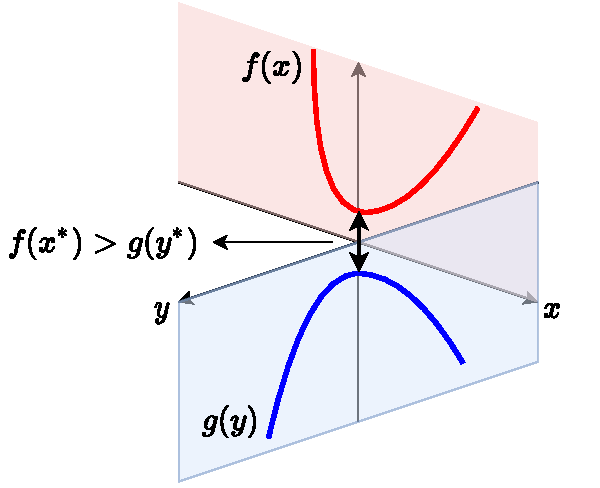
\includegraphics[width=\linewidth]{./figures/weak_dual.pdf}
      \captionsetup{justification=centering}
      \caption{Weak duality.}
    \end{subfigure}
    \hfill
    \begin{subfigure}{.48\textwidth}
      \centering
      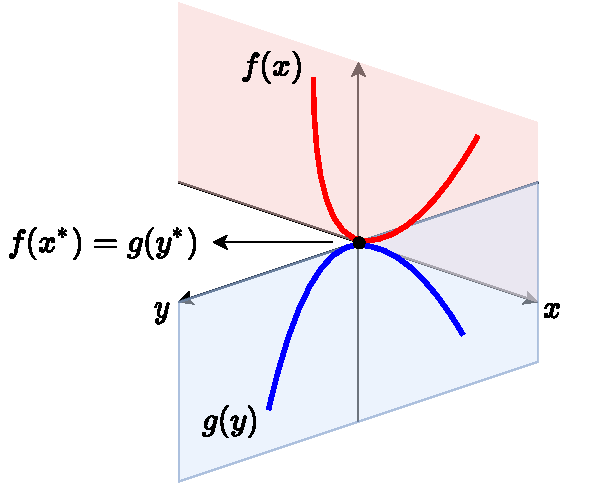
\includegraphics[width=\linewidth]{./figures/strong_dual.pdf}
      \captionsetup{justification=centering}
      \caption{Strong duality.}
    \end{subfigure}
    \captionsetup{justification=centering}
    \caption{Geometric illustration of weak and strong duality.}
    \label{fig:duality}
\end{figure}

\begin{theorem}[Duality theory~\protect{\citep[Theorem~11.39]{rockafellar1998variational}}] Consider the primal-dual pair:~\eqref{prob:general_primal} and~\eqref{prob:general_dual}, where $F: \Re^n \times \Re^m \to \Re$ is a proper, closed and convex function. The following properties hold. 
    \begin{itemize}
        \item \textbf{Weak duality}. The inequality $v_F(0) \geq v_F^{**}(0)$ always holds. 
        \item \textbf{Strong duality}. If $0 \in \ri\dom v_F \cup \ri\dom v_F^{**}$, then $v_F(0) = v_F^{**}(0)$. 
        \item \textbf{Optimal solutions.} If the strong duality holds with finite optimal values, then the following characterizations of the optimal solutions to the primal-dual pair are equivalent
            \begin{align}
                (x^*, 0) &\in \partial F^*(0,y^*); \\
                (0, y^*) &\in \partial F(x^*,0); \\
                v_F(0) = F^*(x^*, 0) &= -F^*(0,y^*) = v_F^{**}(0).
            \end{align}
    \end{itemize}
\end{theorem}

The perturbation function $F$ plays an important role in Fenchel-Rockafellar duality theory. Different choices of the perturbation function will lead to different dual problems. In the rest of this section, we will interpret three widely used primal-dual pairs: Lagrangian dual, Fenchel-Rockafellar dual and gauge dual, under this perturbation framework.  


\subsection{Lagrangian duality}
Consider the general constrained convex optimization problem:
\begin{equation} \label{prob:general_constrained} 
    \minimize{x \in \Re^n} f(x) \st c_i(x) \leq 0 \enspace \forall i = 1, \dots, m,
\end{equation}
where $f:\Re^n\to\Re$ and $c_i:\Re^n\to\Re$ for all $i\in[m]$ are convex functions. In this case, the perturbation function is defined as 
\begin{equation}
    F(x, u) = f(x) + \sum_{i = 1}^m \delta_{\leq 0}(c_i(x) + u_i).
\end{equation}
Then we can derive the corresponding conjugate function as 
\begin{align*}
    -F^*(0, y) &= -\sup_{x\in\Re^n, u\in\Re^m} \ip{0}{x} + \ip{y}{u} - F(x,u)
             \\&= -\sup_{x\in\Re^n, w\in\Re_+^m} \sum_{i=1}^m \ip{y_i}{- c_i(x) - w_i} - f(x)
             \\&= 
             \begin{cases}
                 \inf_{x\in\Re^n} f(x) + \sum_{i=1}^m \ip{y_i}{c_i(x)} & \text{if} y \in\Re_+^m \\
                 -\infty & \text{otherwise}.
             \end{cases}
\end{align*}
Therefore, the Lagrangian dual to problem~\eqref{prob:general_constrained} is given by
\begin{equation} \label{prob:general_constrained_dual}
    \maximize{y\in\Re_+^m} \minimize{x \in \Re^n} f(x) + \sum_{i=1}^m \ip{y_i}{c_i(x)}.
\end{equation}
The following theorem, summarized by \citet{boyd:2004}, characterizes the duality correspondence for the Lagrangian primal-dual pair. 

\begin{theorem}[Lagrangian duality theory~\protect{\citep[Section~5.3]{boyd:2004}}] 
    Let $p^*$ and $d^*$ denote respectively the optimal values for the Lagrangian primal-dual pair:~\eqref{prob:general_constrained} and~\eqref{prob:general_constrained_dual}. 
    \item \textbf{Weak duality}. $p^* \geq d^*$. 
    \item \textbf{Strong duality}. 
    If there exist an interior-point feasible point $\hat x$ for the primal problem~\eqref{prob:general_constrained}, i.e. $c_i(\hat x) < 0$ for $i = 1,\dots,m$, then $p^* = d^*$. Furthermore, let $x^*$ and $y^*$ denote respectively the optimal solutions to the primal-dual pair:~\eqref{prob:general_constrained} and~\eqref{prob:general_constrained_dual}, then 
    \[y_i^*c_i(x^*) = 0 \enspace \forall i = 1,\dots,m.\]
\end{theorem}


\subsection{Fenchel-Rockafellar duality}
Consider the following optimization problem 
\begin{equation} \label{prob:general_fenchel} 
    \minimize{x \in \Re^n} f(x) + g(Mx),
\end{equation}
where $f:\Re^n\to\Re$ and $g:\Re^m\to\Re$ are closed convex functions, and $M:\Re^n\to\Re^m$ is a linear operator. In this case, the perturbation function is defined as 
\begin{equation}
    F(x, u) = f(x) + g(Mx + u).
\end{equation}
Then we can derive the corresponding conjugate function as
\begin{align*}
    -F^*(0, y) &= -\sup_{x\in\Re^n, u\in\Re^m} \ip{0}{x} + \ip{y}{u} - f(x) - g(Mx + u)
             \\&= -\sup_{x\in\Re^n} \left\{\sup_{u\in\Re^m} \ip{y}{Mx + u} - g(Mx + u)\right\} - f(x) - \ip{y}{Mx}
             \\&= - g^*(y) - \sup_{x\in\Re^n}\ip{-M^*y}{x} - f(x) 
             \\&= - g^*(y) - f(-M^*y).
\end{align*}
Therefore, the Fenchel-Rockafellar dual to problem~\eqref{prob:general_fenchel} is given by
\begin{equation} \label{prob:general_fenchel_dual}
    \maximize{y\in\Re^m} - g^*(y) - f(-M^*y).
\end{equation}
The following theorem, developed by \citet{rockafellar1970convex}, characterizes the duality correspondence for the Fenchel-Rockafellar primal-dual pair. 

\begin{theorem}[Fenchel-Rockafellar duality theory~\protect{\citep[Corollary 31.2.1]{rockafellar1970convex}}] 
    Let $p^*$ and $d^*$ denote respectively the optimal values for the Fenchel-Rockafellar primal-dual pair:~\eqref{prob:general_fenchel} and~\eqref{prob:general_fenchel_dual}. 
    \item \textbf{Weak duality}. $p^* \geq d^*$. 
    \item \textbf{Strong duality}. 
    If $0\in\int(\dom g - M\dom f)$, then $p^* = d^*$. Furthermore, let $x^*$ and $y^*$ denote respectively the optimal solutions to the primal-dual pair:~\eqref{prob:general_fenchel} and~\eqref{prob:general_fenchel_dual}, then the following relationships hold
    \begin{align*}
          y^* &\in \partial g(Mx^*) \cap (M^*)^{-1}\partial f(x^*) \tand
        \\x^* &\in \partial f^*(-M^*y^*)\cap M^{-1}\partial g^*(y^*).
    \end{align*}
\end{theorem}




\subsection{Gauge duality}
Consider the following gauge optimization problem 
\begin{equation} \label{prob:general_gauge} 
    \minimize{x \in \Re^n} \gauge\Cs(x) \st Mx = b,
\end{equation}
where $\Cscr\subseteq\Re^n$ is a convex set and $\gauge\Cs$ is the corresponding gauge function, $M:\Re^n\to\Re^m$ is a linear operator, and $b\in\Re^m$ is a vector. By setting 
$\lambda \coloneqq 1/\gauge\Cs(x)$ and $w \coloneqq \lambda x$, problem~\eqref{prob:general_gauge} can be expressed as 
\begin{equation} \label{prob:general_gauge2} 
    \inf_{\lambda > 0, w \in \Re^n} \frac{1}{\lambda} \st w \in \Cscr \tand Mw = \lambda b.
\end{equation}
Note that minimizing $1/\lambda$ is equivalent to minimizing $-\lambda$ for $\lambda \geq 0$. In this case, the perturbation function is defined as 
\begin{equation}
    F(\lambda, w, u) = -\lambda + \delta\Cs(w) + \delta_{\{0\}}(\lambda b - Mw + u) + \delta_{\geq 0}(\lambda). 
\end{equation}
Then we can derive the corresponding conjugate function as
\begin{align*}
    -F^*(0, y) &= -\sup_{\lambda\in\Re, w\in\Re^n, u\in\Re^m} \ip{y}{u} + \lambda - \delta\Cs(w) - \delta_{\{0\}}(\lambda b - Mw + u) - \delta_{\geq 0}(\lambda)
    \\&= -\sup_{\lambda\in\Re, w\in\Re^n} \lambda - \delta\Cs(w) - \delta_{\geq 0}(\lambda) - \ip{\lambda b - Mw}{y}
    \\&= -\sup_{\lambda\geq 0} \delta\Cs^*(M^*y) + \lambda ( 1 - \ip{b}{y} )
    \\&= 
        \begin{cases}
            -\delta\Cs^*(M^*y) & \text{if} \ip{b}{y} \geq 1 \\
            -\infty & \text{otherwise}.
        \end{cases}
\end{align*}
Therefore, the gauge dual to problem~\eqref{prob:general_gauge} is given by
\begin{equation} \label{prob:general_gauge_dual}
    \maximize{y\in\Re^m} -\delta\Cs^*(M^*y) \st \ip{b}{y} \geq 1.
\end{equation}
The following theorem, developed by \citet{friedlander2014gauge}, characterizes the duality correspondence for the gauge primal-dual pair. 

\begin{theorem}[Gauge duality theory~\protect{\citep[Theorem~5.1 and Corollary~5.2]{friedlander2014gauge}}] 
    Let $p^*$ and $d^*$ denote respectively the optimal values for the gauge primal-dual pair:~\eqref{prob:general_gauge} and~\eqref{prob:general_gauge_dual}. 
    \item \textbf{Weak duality}. If both primal problem~\eqref{prob:general_gauge} and dual problem~\eqref{prob:general_gauge_dual} are feasible, then $p^* d^* \geq 1$. 
    \item \textbf{Strong duality}. If either primal problem~\eqref{prob:general_gauge} or dual problem~\eqref{prob:general_gauge_dual} is strictly feasible and the other is feasible, then $p^* d^* = 1$. Furthermore, let $x^*$ and $y^*$ denote respectively the optimal solutions to the primal-dual pair:~\eqref{prob:general_gauge} and~\eqref{prob:general_gauge_dual}, then 
    \[\ip{x^*}{M^*y^*} = \gauge\Cs(x^*)\delta\Cs^*(M^*y^*).\]
    
\end{theorem}

\section{Structured optimization} \label{sec:1-3}

Convex optimization provides a valuable computational framework that renders many problems tractable because of the range of powerful algorithms that can be brought to the task. The key is that a specific mathematical structure, i.e., the convexity of the functions and sets defining the problem—opens an enormous range of theoretical and algorithmic tools that lend themselves astonishingly well to computation. However, there are limits to the scalability of general-purpose algorithms for convex optimization. As has been recognized in the optimization and related communities for at least the past decade, significant efficiencies can be gained by acknowledging the latent structure in the solution itself, coupled with the overarching structure provided by convexity.

Structured optimization proceeds by using a prescribed set of atoms to assemble an optimal solution. The atomic decomposition of a vector $x\in\Re^n$ with respect to an atomic set
$\Ascr\subset\Re^n$ is given by the weighted superposition
\begin{equation} \label{eq:atomic-decomp}
  x = \sum_{a\in\Ascr} c_a a, \quad c_a\ge0 \quad \forall a\in\Ascr.
\end{equation}
Each coefficient $c_a$ in the atomic decomposition measures the contribution of
the corresponding atom $a$ toward the representation of $x$. Intuitively, an
atomic decomposition reveals structural information implicit in a vector, with
large coefficients in the decomposition indicating the more essential
structures.

Within the context of an optimization problem, the atomic decomposition reveals
structural elements most essential in the minimization process.
In the simplest case, the atoms $\Ascr$ may be formed from the collection of
signed canonical unit vectors $\{\pm e_1,\ldots,\pm e_n\}$, which leads to the
atomic decomposition
\[
  x = \sum_{j=1}^n c_j a_j,
  \quad
  c_j: = |x_j|,
  \quad
  a_j:= (\sgn x_j)\cdot e_j.
\]
Trivially, the essential atoms thus correspond to the variables $x_j$ in
the vector $x=(x_1,\ldots,x_n)$ with nonzero magnitude.

This generic model for atomic decompositions was promoted by~\citet{cds98} in the context of sparse signal decomposition, and more recently, by~\citet{chandrasekaran2012convex}, who were concerned with obtaining sparse solutions to linear inverse problems. 

In this thesis, we want to answer the question of determining which of the atoms in the atomic set $\Ascr$ are essential to the atomic decomposition of $x$, and conversely, which atoms can be safely ignored. In \autoref{ch:Dual-Struc-Opt}, we study the atomic decomposition framework from a dual perspective. Polarity, which extends the familiar notion of orthogonality from linear sets to general convex sets, plays a special role in a simple and geometric form of convex duality. This duality correspondence yields a general notion of alignment that leads to an intuitive and complete description of how atoms participate in the final decomposition of the solution. The resulting dual perspective leads to variations of existing algorithms effective for large-scale problems. We illustrate these ideas with many examples, including applications in matrix completion and morphological component analysis. We further show that this dual alignment property allows us to design new structured optimization models for real-world applications and develop efficient and scalable algorithms for structured optimization problems. We briefly introduce the roadmap below. 

In \autoref{ch:App-Sig-Demix}, we study the structured signal demixing problem which seeks to separate a superposition of multiple signals into its constituent structural components. We propose a two-stage approach that first decompresses and subsequently deconvolves the noisy and undersampled observations of the superposition. Probabilistic error bounds are given on the accuracy with which this process approximates the individual signals. The theory of polar convolution of convex sets developed by~\citet{friedlander2019polarconvolution}, and the dual alignment property developed in \autoref{ch:Dual-Struc-Opt} play central roles in the analysis and solution process. If the measurements are random and the noise is bounded, this approach stably recovers low-complexity and mutually incoherent signals, with high probability and with optimal sample complexity. Numerical experiments on both real and synthetic data confirm the theory and the efficiency of the approach.

In \autoref{ch:App-Primal-Retrieval}, we study the structured data-fitting problem, which is prevalent in machine learning and data mining. In practice, people solve the corresponding structured convex relaxations. When tackling high-dimensional structured optimization problems, dual-based algorithms are usually preferred over primal-based algorithms as dual variables usually live in a much lower-dimensional space than primal variables. One common issue of dual-based algorithms is that they still need to translate dual variables to primal variables at some point. How to retrieve a near-optimal primal variable efficiently with a provable guarantee is thus crucial for the success of dual approaches. We present a simple and computationally cheap strategy for retrieving a primal variable from any feasible dual variable, which is based on the dual alignment property developed in \autoref{ch:Dual-Struc-Opt}. Theoretically, we show that our proposed strategy is capable of obtaining a near-optimal primal variable given a dual-based algorithm converging to the optimal dual solution. Numerical experiments on real-world datasets support our analysis.

In \autoref{ch:App-AtomicOpt}, we introduce our open-source package \texttt{AtomicOpt.jl} for solving a class of structured optimization problems, which is written in the Julia programming language~\citep{bezanson2017julia}. Our design depends on the level-set method~\citep{aravkin2016levelset}, a dual version of the conditional-gradient method~\cite{jaggi2013revisiting,frank1956algorithm,dunn1978conditional}, and the primal-retrieval strategy developed in~\autoref{ch:App-Primal-Retrieval}. The worst-case computational complexity of our algorithm is sublinear in the required accuracy. All the numerical experiments conducted in~\autoref{ch:Dual-Struc-Opt},~\autoref{ch:App-Sig-Demix} and~\autoref{ch:App-Primal-Retrieval} are reproducible via this package. 



 

\section{Federated learning} \label{sec:1-4}

With the development of artificial intelligence, people recognize that many powerful machine learning models are driven by large decentralized datasets, e.g., AlphaGo~\citep{silver2016mastering} and AlexNet~\citep{krizhevsky2012imagenet}. In many industry-scale applications, training data is distributed in the form of silos, that is, training data is obtained and maintained by many data owners instead of being centralized at the place of a single owner or a data center. Because of industrial competition, privacy concerns, legal restrictions, and many other possible reasons, integrating or centralizing data from different sources faces enormous resistance and is often even infeasible~\citep{li2020review}. Federated learning, originally proposed by~\citet{federated2016}, is promising for training machine learning models on distributed data sources. It facilitates collaboration among a group of data owners (aka.~``clients'') and, at the same time, preserves their privacy. The central idea of federated learning is to periodically aggregate local models from clients to produce a more general and capable global model.

Federated learning can be further be classified into two main categories: horizontal federated learning and vertical federated learning~\cite{yang2019federated}. Horizontal federated learning refers to the scenarios where various clients' data sets share the same feature space but have separate sample IDs, and vertical federated learning refers to the scenarios where data sets owned by different clients share the identical sample IDs but have distinctive features. A simple characterization is shown in \autoref{fig:hfl_and_vfl}. 

\begin{figure}[t] 
    \begin{subfigure}{.48\textwidth}
      \centering
      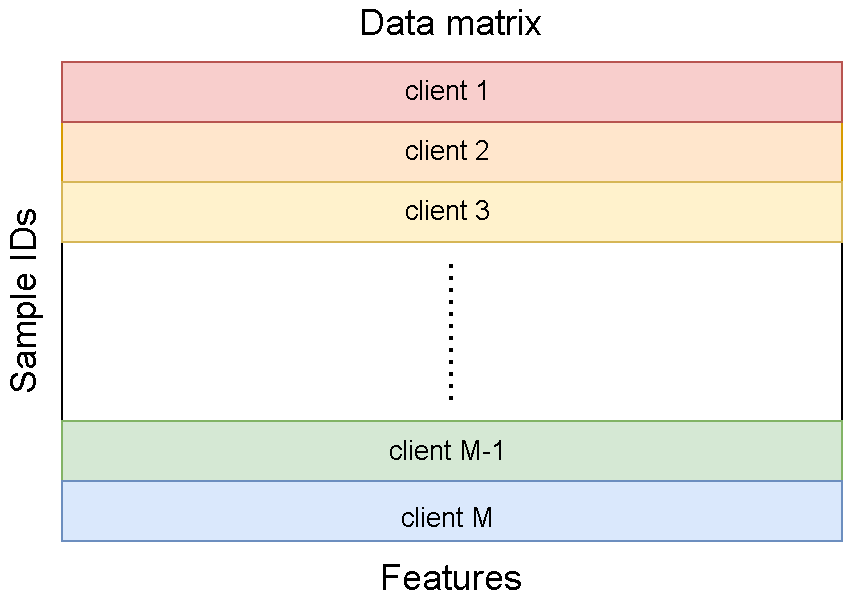
\includegraphics[width=\linewidth]{./figures/hfl_illustration.pdf}
      \captionsetup{justification=centering}
      \caption{Horizontal federated learning.}
      \label{fig:hfl}
    \end{subfigure}
    \hfill
    \begin{subfigure}{.48\textwidth}
      \centering
      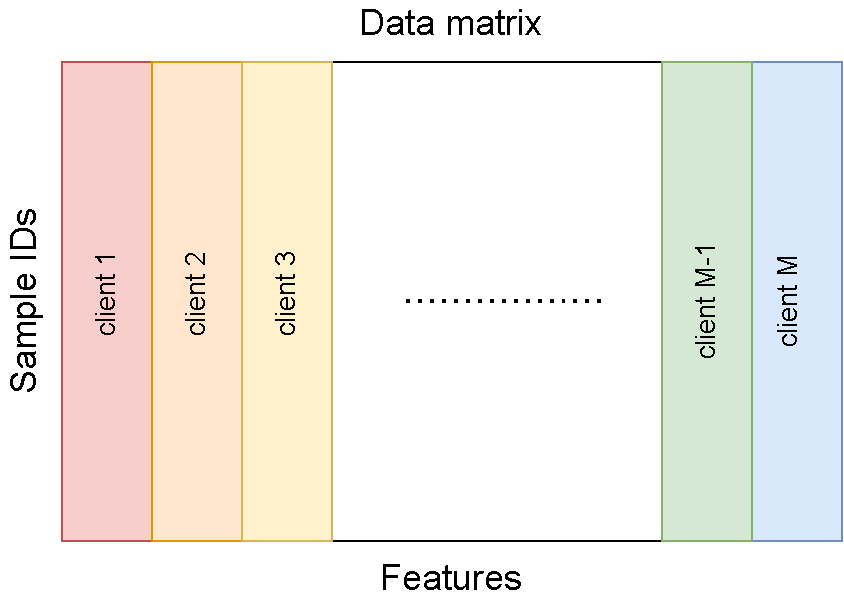
\includegraphics[width=\linewidth]{./figures/vfl_illustration.pdf}
      \captionsetup{justification=centering}
      \caption{Vertical federated learning.}
      \label{fig:vfl}
    \end{subfigure}
    \captionsetup{justification=centering}
    \caption{Characterization of horizontal and vertical federated learning.}
    \label{fig:hfl_and_vfl}
\end{figure}

This thesis shows that duality can be utilized to develop efficient and scalable algorithms for the optimization problem arising from federated learning. Besides, we show that structured optimization techniques can play an essential role in designing fair contribution valuation rules in federated learning. We briefly introduce the roadmap below. 

\subsection{Federated optimization} \label{sec:1-4-1}

A federated learning system is often composed of two components: clients and a central server at the physical level. The learning process in federated learning can be formulated as a distributed optimization problem, also known as federated optimization. As characterized and formalized by~\citet{wang2021field},~\citet{li2020federated} and~\citet{li2019convergence}, several essential characteristics distinguish FO from standard machine learning and distributed optimization. 

\begin{assumption}[Governing assumptions for federated optimization] \label{assum:govern}
The following assumptions hold for federated optimization. 
  \begin{itemize}
    \item \textbf{Slow Communication.}  Communication between clients and a central server is assumed to be the main bottleneck and dominates any computational work done at each of the clients. 
    \item \textbf{Data Privacy.} Clients want to keep their local data private, i.e., their data can not be accessed by any other client nor by the central server.
    \item \textbf{Data heterogeneity.} The training data are not independent and identically distributed (i.i.d.). In other words, a client’s local data cannot be regarded as samples drawn from single overall distribution.
    \item \textbf{Partial Participation.} Unlike traditional distributed learning systems, an FL system does not have control over individual client devices, and clients may have limited availability for connection. 
\end{itemize}
\end{assumption}

In \autoref{ch:Dual-Fed-Opt}, we study the federated optimization problem from a dual perspective. We propose a new algorithm termed federated dual coordinate descent (FedDCD), which is based on a type of coordinate descent method developed by \citet{necoara2017random}.  Additionally, we
enhance the FedDCD method with inexact gradient oracles and Nesterov's acceleration. We demonstrate
theoretically that our proposed approach achieves better convergence rates than the state-of-the-art
primal federated optimization algorithms under certain situations. Numerical experiments on real-world
datasets support our analysis.

\subsection{Contribution valuation in federated learning} \label{sec:1-4-2}

The effectiveness of federated learning depends on the active participation of motivated clients. Another important question in federated learning is how to ensure the clients’ long-term engagement, and how to motivate more clients' participation. One possible practical solution is to recompense the participated clients according to their contribution. 

Shapley value~\cite{shapley201617} is a classical measure originates from cooperative game theory to fairly assess contributions by participants in a coalition. 
The Shapley value of a participant is defined as the expectation of the marginal contribution of the participant over all possible subsets of the other participants. Shapley value is the unique measure that satisfies the four fundamental requirements of fairness proposed by Shapley~\cite{shapley201617}: balance, symmetry, zero element and additivity, which we formally define bellow. 

\begin{definition} \label{def:shapley}
    Supporse there are $M$ clients and there is a black-box utility function $U:2^{[M]} \to \Re$ such that for any subset of clients $S \subseteq [M]$, the function $U(S)$ returns a utility score of the model collaboratively trained by the clients in $S$, such as the performance of the model. Let $v: [M] \to \mathbb{R}$ be the evaluation metric associated with the utility function $U$. The metric $v$ is called \emph{Shapley-fair} with respect to $U$ if it satisfies the following for fundamental requirements
    \begin{enumerate}
        \item \textbf{Symmetry.} For any two clients $i, j \in [M]$, if for any subset of clients $S \subseteq [M] \setminus \{i,j\}$, $U(S \cup \{i\}) = U(S \cup \{j\})$, then $v(i) = v(j)$. 
        \item \textbf{Zero element.} For any client $i \in [N]$, if for any subset of clients $S \subseteq [M] \setminus \{i\}$, $U(S \cup \{i\}) = U(S)$, then $v(i) = 0$.
        \item \textbf{Additivity.} If the utility function $U$ can be expressed as the sum of separate utility functions, namely $U = U_1 + U_2$ for some $U_1, U_2 : 2^I \to \mathbb{R}$, then for any client $i \in [M]$, $v(i) = v_1(i) + v_2(i)$, where $v_i$ and $v_2$ are the evaluation metrics associated with the utility functions $U_1$ and $U_2$, respectively. 
        \item \textbf{Balance.}  $U([M]) = \sum_{i \in [M]} v(i)$.
    \end{enumerate}
\end{definition}

Under the federated learning setting, a utility function is usually defined as the model performance on a data set. The symmetry requires that the same contributions to the performance should receive the same evaluation, which implies that clients with same local data sets should receive same evaluation. The zero element requires that no contribution, no value is recognized. The additivity requires that if there are multiple tasks and thus multiple test data sets, then the contributions of any client with respect to the test data sets can be expressed as the sum of the contributions with respect to those different tasks and test data sets. Note that, although balance is a necessary condition in many economic contests because it ensures payment is fully distributed to all clients, it is irrelevant in the context of federated learning because we are only concerned about the relative contributions of clients. It is shown~\cite{dubey1975uniqueness,ghorbani2019data} that if the data valuation metric $v$ satisfies symmetry, zero element, and additivity, then $v$ must have the form
\begin{equation} \label{eq:shapley}
    v(i) = c \sum\limits_{S \subseteq I \setminus\{i\}} \frac{1}{\binom{N-1}{|S|}} \left[U(S\cup\{i\}) - U(S)\right],
\end{equation}
for some positive constant $c$.  

Although Shapley value has many desirable properties, evaluating Shapley value in federated learning requires exhaustive retraining and evaluating the model on every subset of clients. The costs of communication and time may be prohibitive in practice~\cite{song2019profit}. To tackle this challenge, some variations inspired by Shapley value were developed. Federated Shapley value (FedSV), recently proposed by \citet{wang2020principled}, is a measure for valuating contribution under the framework of horizontal federated learning. The key idea is to compute the Shapley values for clients in each round of training and then report the summation over all the rounds as the final results. This design cleverly avoids model retraining. However, there are still factors of potential unfairness in the design of FedSV because two data owners with the same local data may not receive the same evaluation. 

In \autoref{ch:Val-HFL}, we propose a new measure called completed federated Shapley value (ComFedSV) for contribution valuation in horizontal federated learning, which improves the fairness of FedSV. The design depends on completing a matrix consisting of all the possible contributions by different subsets of the data owners. It is shown under mild conditions that this matrix is approximately low-rank by leveraging concepts and tools from structured optimization. Both theoretical analysis and empirical evaluation verify that the proposed measure does improve fairness in many circumstances.

In \autoref{ch:Val-VFL}, we extend the idea of FedSV to vertical federated learning. We propose a contribution valuation metric called vertical federated Shapley value (VerFedSV), which utilizes tools from structured optimization. We show that VerFedSV not only satisfies many desirable properties for fairness but is also efficient to compute, and can be adapted to both synchronous and asynchronous vertical federated learning algorithms. Both theoretical analysis and extensive experimental results verify the fairness, efficiency, and adaptability of VerFedSV.






%    2. Main body
% Generally recommended to put each chapter into a separate file
%\include{relatedwork}
%\include{model}
%\include{impl}
%\include{discussion}
%\include{conclusions}

%    3. Notes
%    4. Footnotes

%    5. Bibliography
\begin{singlespace}
\raggedright
\bibliographystyle{abbrvnat}
\bibliography{biblio}
\end{singlespace}

\appendix
%    6. Appendices (including copies of all required UBC Research
%       Ethics Board's Certificates of Approval)
%\include{reb-coa}	% pdfpages is useful here
\include{appendix}

\backmatter
%    7. Index
% See the makeindex package: the following page provides a quick overview
% <http://www.image.ufl.edu/help/latex/latex_indexes.shtml>


\end{document}
